\texttt{for loops}\chapter{Evaluation}
\label{sec:evaluation}
% Analyse on expressions instead of statements.
% Statements that contain a block should have not been split as this makes reconstruction very difficult.
Evaluating the success of my solution is difficult. My implemented solution only works for some examples, as only some features of the language are supported. Its focus is on parallelising as much as possible, not necessarily on getting a faster program. To get an idea of how much parallelism was found, the parallel source code was statically examined to find out how many threads and channels are created. These values may be lower than the actual number of threads used, as some thread definitions will be reused (repeated function call, \texttt{for loops}, etc.). Each program was compiled sequentially and in parallel, with and without optimisations.

Two manually written sequential programs were parallelised: a simple example and a password cracker. The dependency tree and schedule are analysed to show how the parallelising compiler works. To test the robustness of the compiler, a collection of automatically generated sequential programs were also parallelised. The output of the parallel version was compared with the sequential version to check that the parallelisms have not semantically changed the program.

\section{Sequential Programs Parallelised}
\subsection{Simple Example}
This simple example is intended to be an easy way to show how the parallelising compiler works. It consists of two independent variables, \texttt{a} and \texttt{b} which are incremented and then printed together. An extra independent print statement is also added at the end to show one potential problem with the dependency analysis.

\begin{code}
    \inputcode{simple-example/main.rs}{}{}
    \caption{A simple example program}
\end{code}

\begin{figure}
    \subcaptionbox{\label{fig:simple-deps}Dependency analysis}%
    [.5\textwidth]{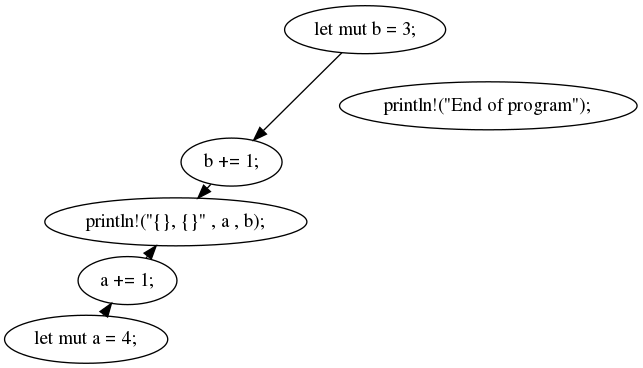
\includegraphics[width=.5\textwidth]{img/simple-example/main-dependency-analysis.png}}
    \subcaptionbox{\label{fig:simple-sch}Schedule}
    [.5\textwidth]{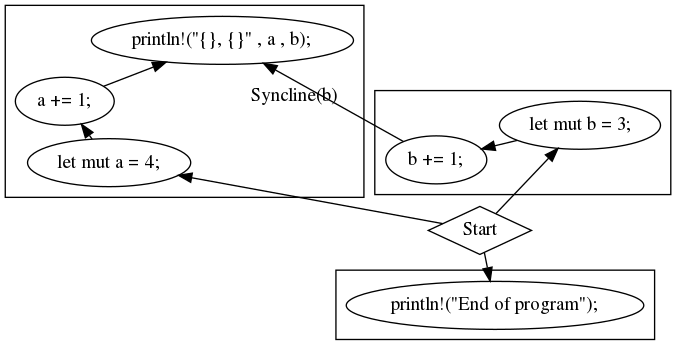
\includegraphics[width=.5\textwidth]{img/simple-example/main-schedule.png}}
    \caption{Main method from the simple example program}
\end{figure}

\autoref{fig:simple-deps} clearly shows \texttt{a} and \texttt{b} do not need to be inter-weaved. It also shows that the \texttt{println!(``End of program");} is completely independent of the other print statement. This may not be intended by the programmer, but there is nothing inside the \texttt{println!} macro which states that they must be called in order (there is no variable linking the two print statements). This could be fixed by forcing non-analysed functions to be executed in order, but it may not be an actual dependency and it would reduce the number of parallelisms detected. Because this dependency is not detected, I sorted the outputs of both sequential and parallel programs so that the order does not matter when comparing program outputs. \autoref{fig:simple-sch} shows that the scheduling algorithm split \texttt{a} and \texttt{b} into separate threads as well as the ``End of program" print statement. The print statement that prints \texttt{a} and \texttt{b} attached itself to the \texttt{a} thread. The \texttt{b} variable is sent along the syncline just before the print.

\subsection{Password Cracker}
A password cracker program is a good target for paralleling. Each word in a dictionary is hashed individually and then compared with the hash of a password that the user is trying to crack. My implementation contains three functions: \texttt{loadDictionary()}, \texttt{hash()} and \texttt{main()}. The \texttt{loadDictionary()} is not analysed here as the parallelising compiler did not make any changes to this function. This program is on the limits of what my parallelising compiler can do in its current state. Some of the code is written in a semi-specific way to get it to parallelise properly.

\subsubsection{Hash Function}
\begin{code}
    \inputcode{password-cracker/main.rs}{27}{37}
    \caption{Hash function of the password cracker program}
\end{code}

The word argument is iteratively hashed $1000$ times with SHA256 from an external crate. If I let the parallelising compiler try to parallelise this loop, it would produce code that does not compile.
\texttt{hasher.result\_str()} returns a \texttt{str} which is normally converted to a \texttt{String}. When run in parallel, it tries to send a \texttt{str} down a syncline which does not work as \texttt{str} does not implement the \texttt{Send} trait.
This could be fixed by storing the type with the variable name instead of relying on type inference. Another reason for disabling parallelisation of this loop is that it would slow down the program. Most of the statements depend on the previous iteration and so no speedup can be achieved here. Line $32$ has no dependencies and could be run in parallel but it is not computationally expensive to call \texttt{Sha256::new()} so it is not beneficial. If some performance analysis technique was implemented, then it would notice that it is a bad idea to parallelise this loop.
To disable parallelisation of this loop, I added \texttt{.rev()} to the range of the loop. This is very hacky, but it breaks one of the extra restrictions I placed on parallelising \texttt{for loops} so it will not be parallelised.

\begin{figure}
    \subcaptionbox{\label{fig:hash-deps}Dependency analysis}%
    [.6\textwidth]{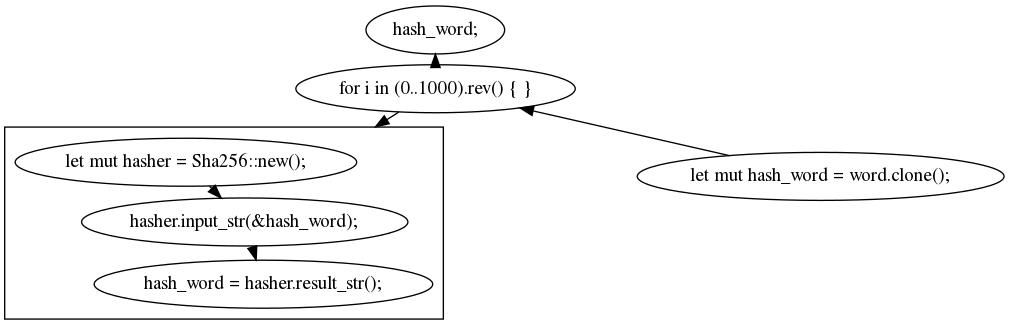
\includegraphics[width=.6\textwidth]{img/password-cracker/hash-dependency-analysis.png}}
    \subcaptionbox{\label{fig:hash-sch}Schedule}
    [.4\textwidth]{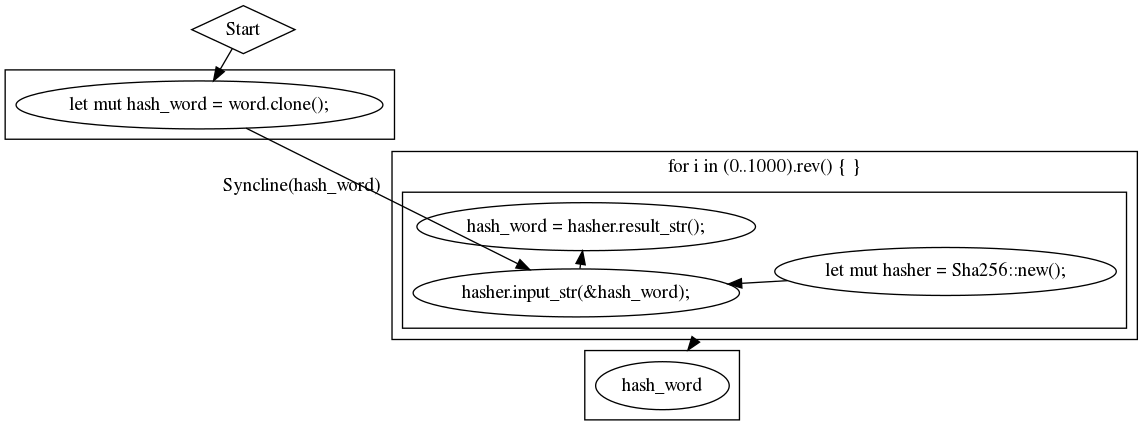
\includegraphics[width=.4\textwidth]{img/password-cracker/hash-schedule.png}}
    \caption{Hash function from the password cracker program}
\end{figure}

\autoref{fig:hash-deps} shows how the inner block is linear for one iteration. The reason that the loop cannot be parallelised effectively is that \texttt{hash\_word} is modified each iteration.
\autoref{fig:hash-sch} shows how linear the iterative hash function is. The only separate thread that is spawned clones the word. The reason that the \texttt{for loop} is not inside the same thread is because the \texttt{hash\_word} dependency is inside the \texttt{for loop}. The condition on the \texttt{for loop} is independent and could be slow and so is parallelised. In reality, parallelising this loop will be much slower due to thread overhead.

\subsubsection{Main Method}
The main method loads the dictionary from a file into a list of strings. Each word in this list is hashed and compared with a password hash. Notice that the \texttt{for loop} is not interrupted when it finds the correct word, or even stored; it is just printed. A timing circuit is placed around the function to print how long it takes to find the password.

\begin{code}
    \inputcode{password-cracker/main.rs}{39}{57}
    \caption{Main method of the password cracker program}
\end{code}

As you can see from the \autoref{fig:pass-deps} and \autoref{fig:pass-sch}, the timing circuit is a completely independent program. This is probably not intended, and it is a similar problem to the \texttt{println!} problem from the simple example. This is a slight difference however, as the order for the time circuit is actually correct but the time that the timing circuit is run is different. There is no real solution I can think of for this issue except hard coding the time crate to be dependent on everything before it and everything after it dependent on it. Hard coding this may be problematic as there may be other functions in other crates which also have similar dependency requirements. I will just remove the timing circuit when comparing the outputs as the time will not be consistent between runs.
The schedule (\autoref{fig:pass-sch}) shows that the \texttt{password\_hash} assignment is placed in its own thread, as the \texttt{for loop} condition is independent. The block inside the \texttt{for loop} does depend on this value, and so a syncline is setup. It is not clear from the schedule above, but the \texttt{for loop} is also parallelised. \autoref{fig:pass-for-sch} shows how the each iteration of the \texttt{for loop} is parallelised and what synclines are required.
The \texttt{dictionary} and \texttt{password\_hash} variables are requested on the first line they are required in the iteration and sent to the next iteration when they are no longer needed. In this case, only one statement uses each external dependency, so it is immediately released. The \texttt{hash} function is computationally expensive, and can only be started once it has access to its word in the dictionary. The dictionary can be passed very quickly through all of the threads, as accessing the element inside a list is very fast. This allows multiple \texttt{hash} functions to be run at the same time. The \texttt{password\_hash} variable is requested after the \texttt{hash} function returns, meaning \texttt{id=1} cannot check whether it is equal to the \texttt{password\_hash} if its \texttt{hash} function returns before \texttt{id=0}.

\begin{figure}
    \begin{subfigure}{\textwidth}
        \centering
        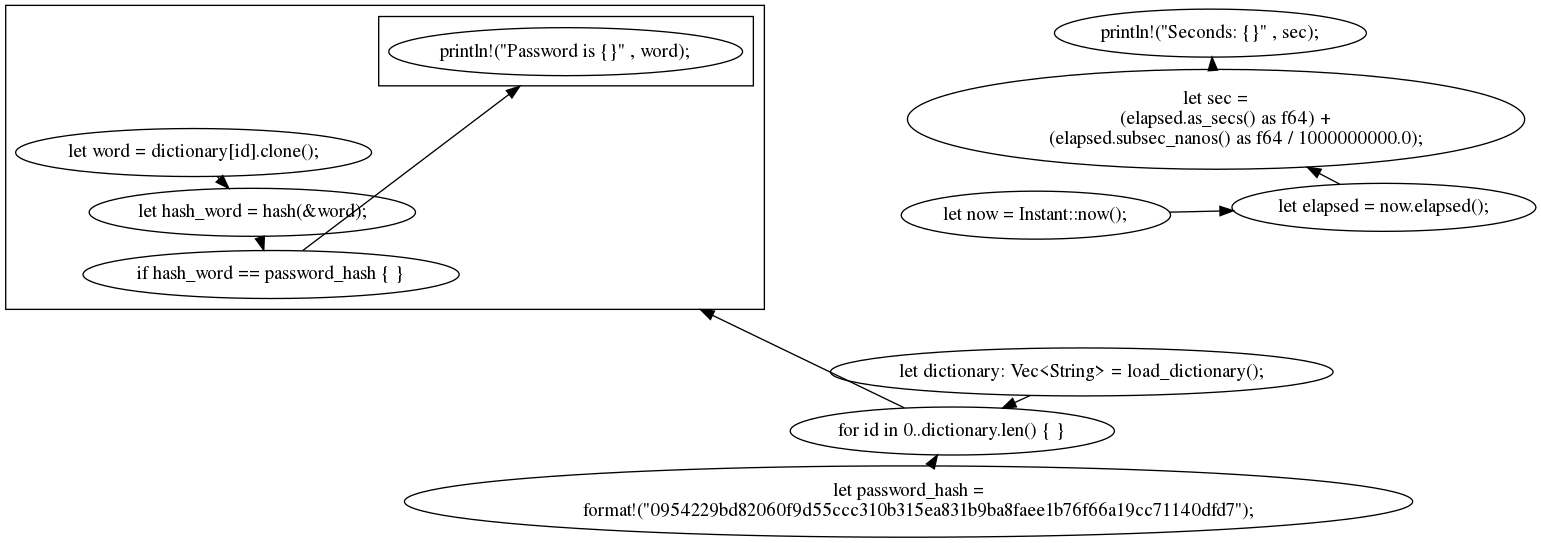
\includegraphics[width=\textwidth]{img/password-cracker/main-dependency-analysis.png}
        \caption{\label{fig:pass-deps}Dependency analysis}
        \vspace{1em}
    \end{subfigure}
    \begin{subfigure}{\textwidth}
        \centering
        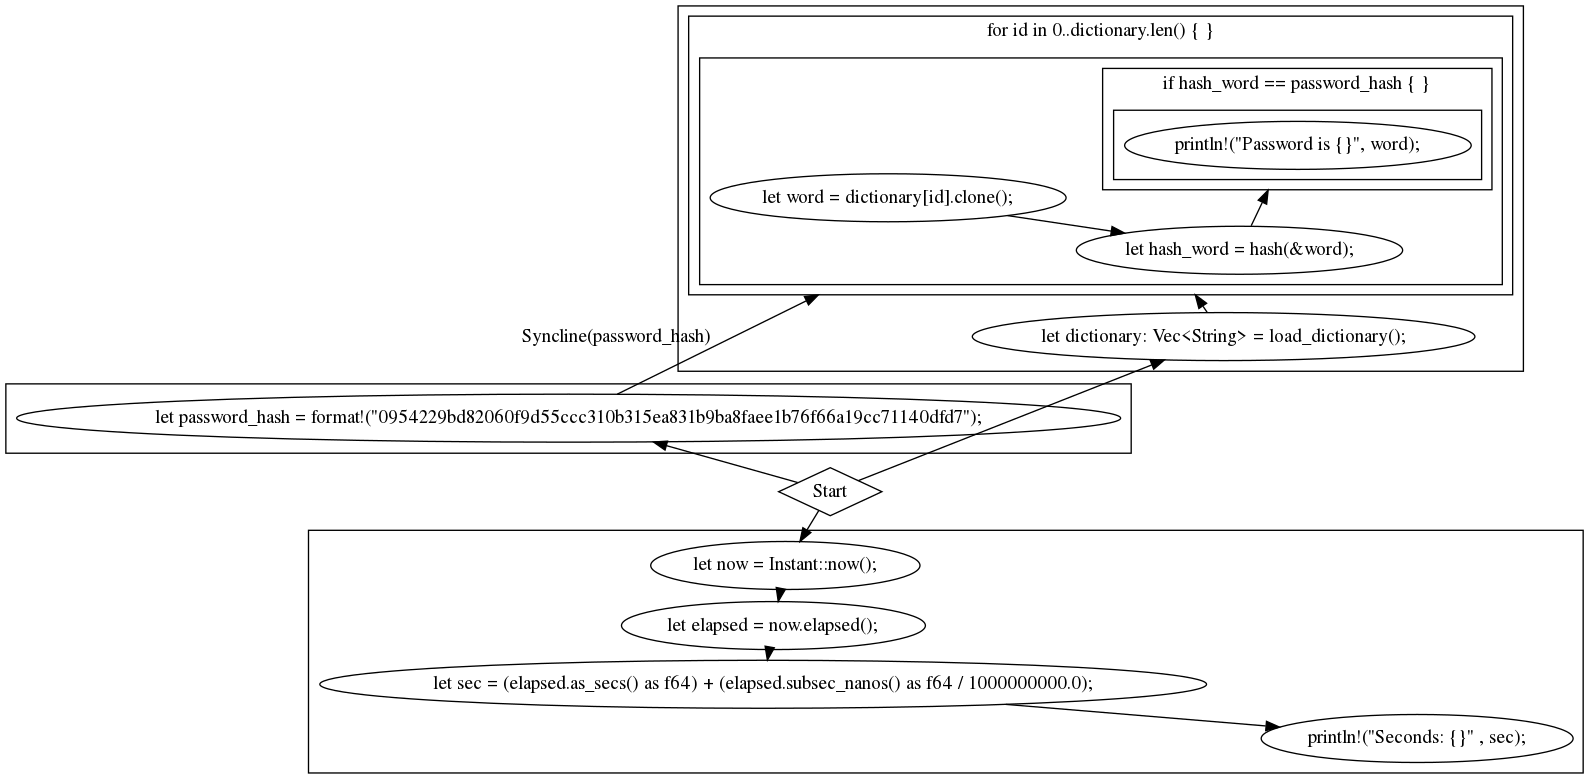
\includegraphics[width=\textwidth]{img/password-cracker/main-schedule.png}
        \caption{\label{fig:pass-sch}Schedule}
    \end{subfigure}
    \caption{Main method from the password cracker program}
\end{figure}

\begin{figure}[H]
    \centering
    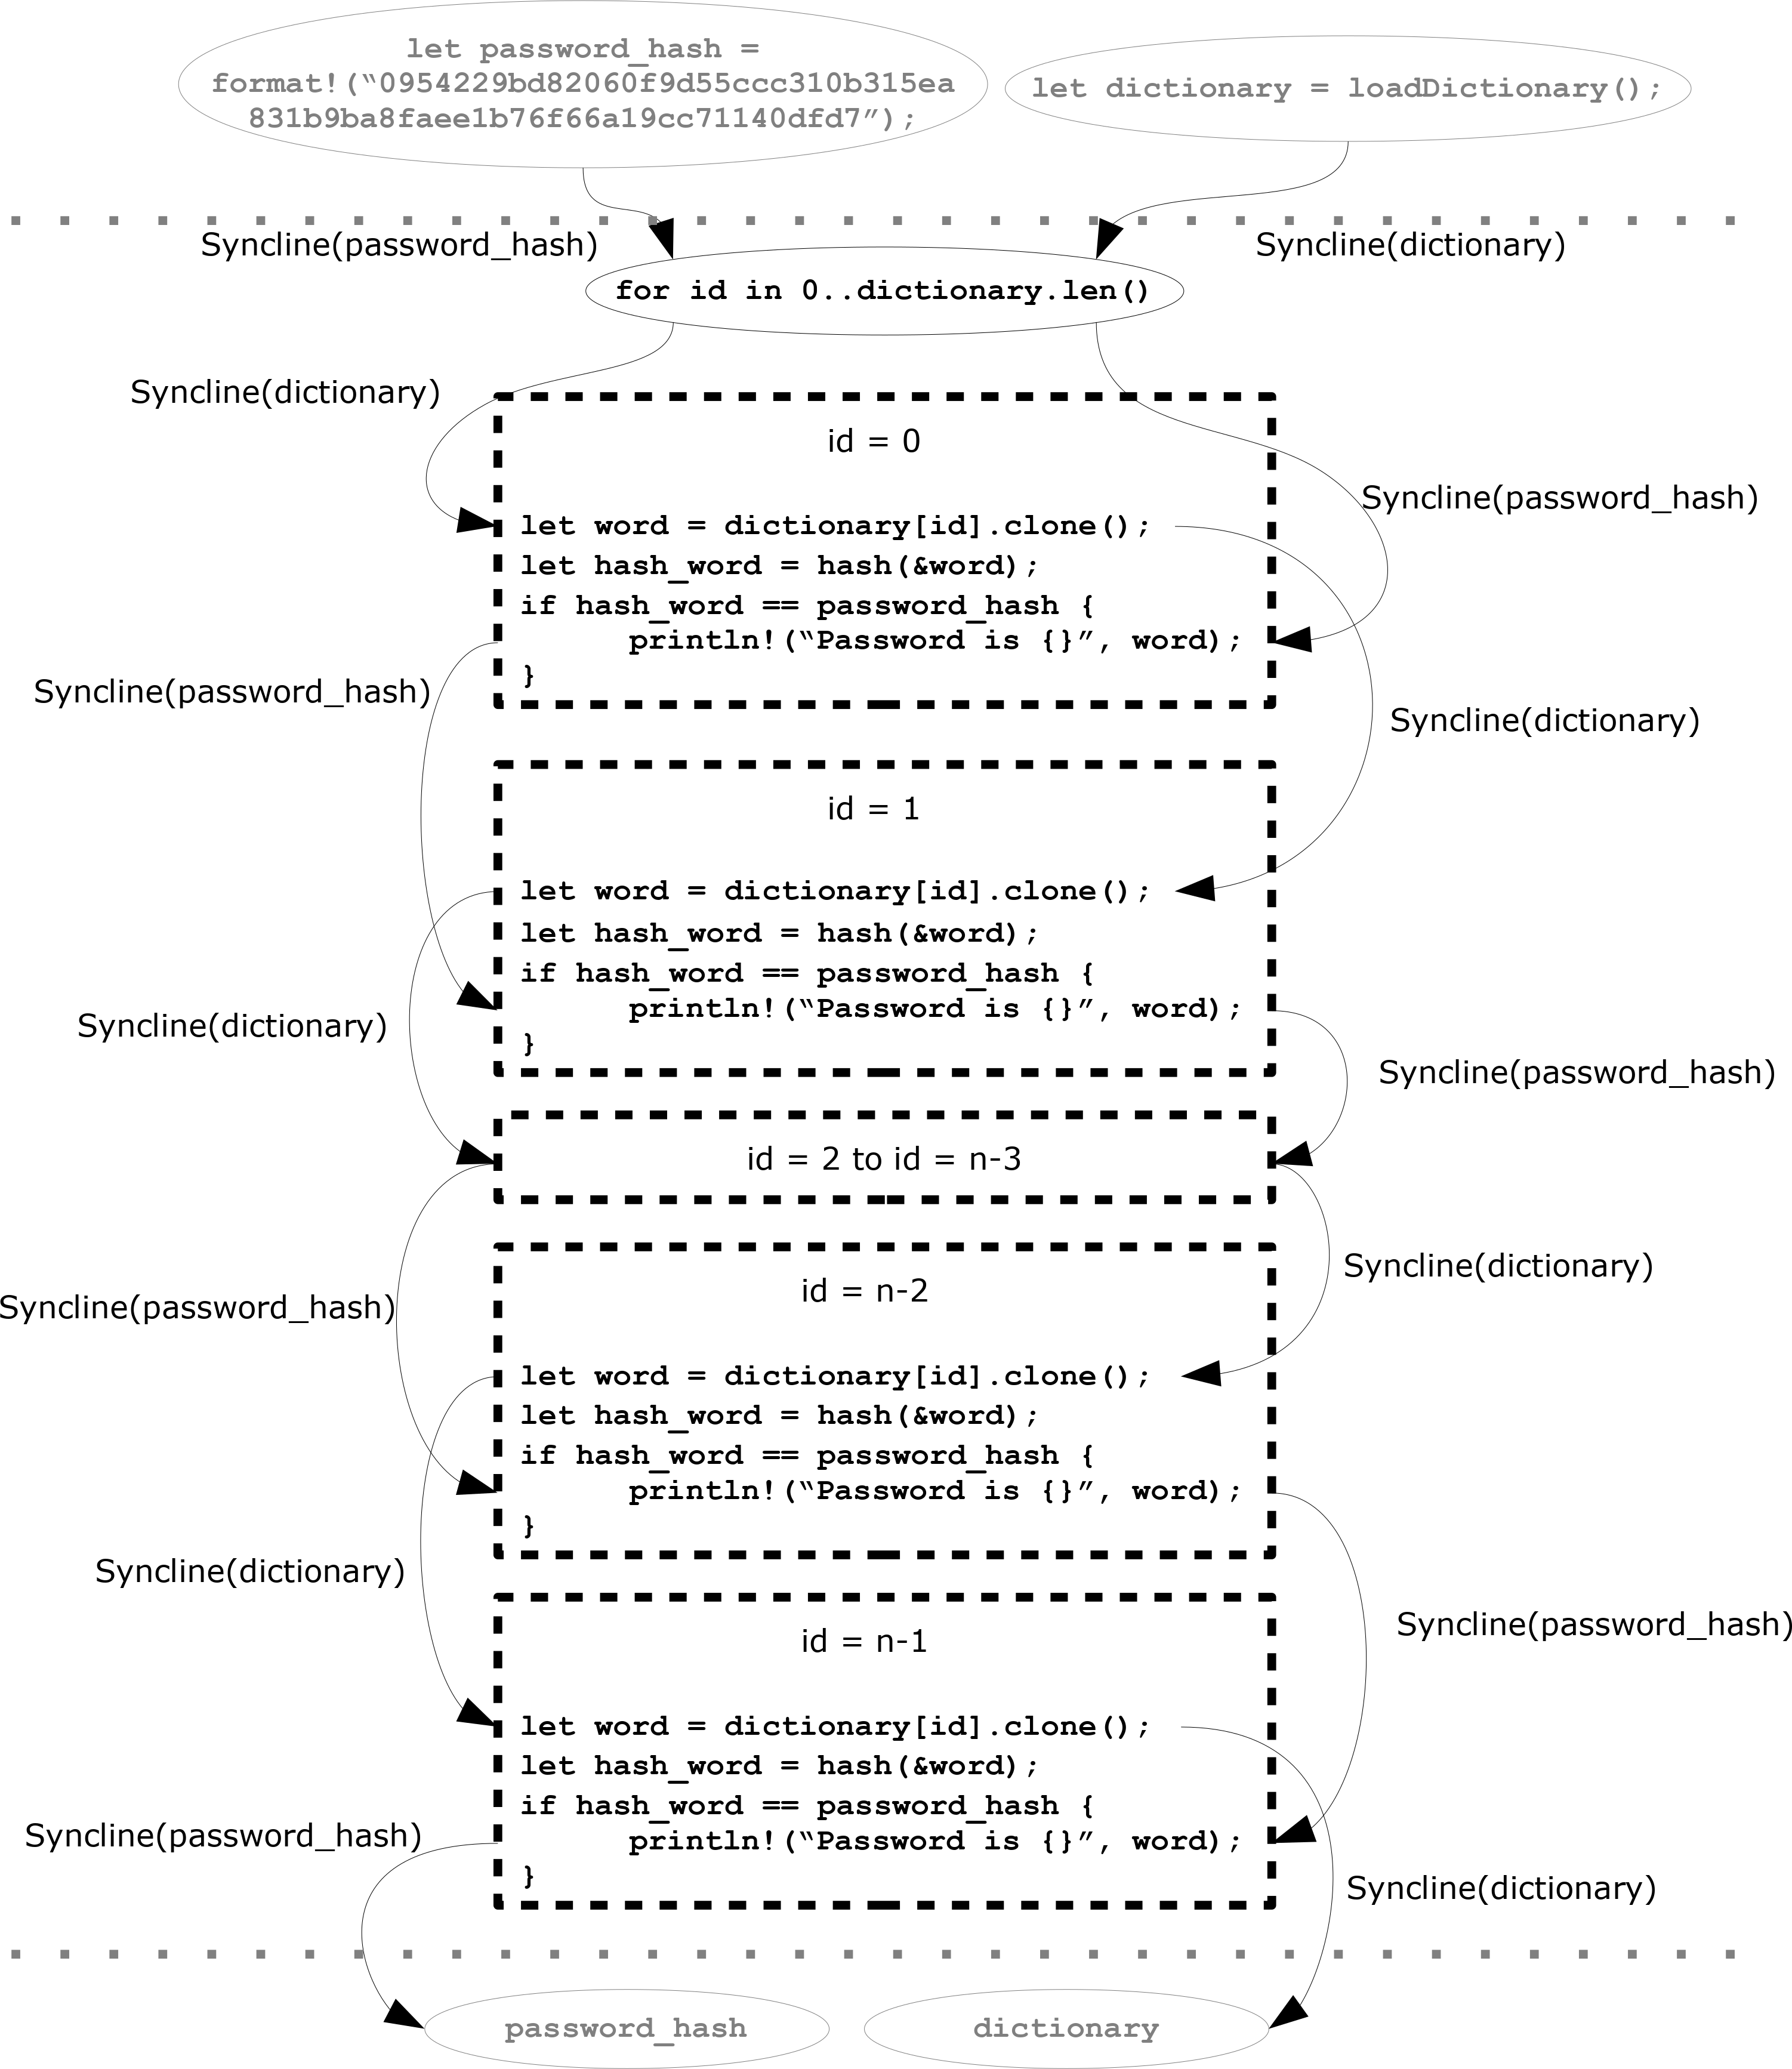
\includegraphics[width=\textwidth]{img/password-cracker/parallel-for.png}
    \caption{\label{fig:pass-for-sch}A schedule to show how the \texttt{for loop} in the main method from the password cracker program is parallelised}
\end{figure}

\subsection{Automatically Generated Sequential Programs}
To verify that the parallelising compiler can parallelise more that the programs shown above, it was tested against a collection of randomly generated sequential programs with increasing complexity. The first set of programs only contained variable creation, variable assignment and printing arbitrary expressions. A list was added at the beginning of the program which puts the command line arguments into an array. This was used to add some consistent dynamic element that the compiler optimisations would not be able to optimise out. The second set of programs added \texttt{for loops} and \texttt{if} statements, which allows for nested blocks. I tested these programs without parallel \texttt{for loop} optimisations enabled. The third set uses the same sequential programs as the second set but has parallel \texttt{for loop} optimisations enabled. The complexity value varies for each program within each set. This affects how many statements are generated in the sequential source code. Listing \autoref{code:genprogram1} is an example of a generated program from the first set. Listing \autoref{code:genprogram2} is an example from the second/third set.

\begin{code}
\begin{minted}{rust}
fn main() {
    let stdin: Vec<i32> = ::std::env::args().skip(1).map(|i| i.parse::<i32>().unwrap()).collect();
    {
        println!("00000000: (stdin[0]) - (stdin[4]) = {:?}", (stdin[0]) - (stdin[4]));
        println!("00000001: (stdin[17]) - (((4) + (1)) - (-4)) = {:?}", (stdin[17]) - (((4) + (1)) - (-4)));
        println!("00000002: (stdin[8]) - (1) = {:?}", (stdin[8]) - (1));
        let mut s: i32 = 0;
        s = stdin[9];
        println!("00000003: ((8) * (9)) - ((s) * (1)) = {:?}", ((8) * (9)) - ((s) * (1)));
        let mut u: i32 = 0;
        println!("00000004: u = {:?}", u);
        let mut a: i32 = 0;
        let mut z: i32 = 0;
        println!("00000005: s = {:?}", s);
        println!("00000006: u = {:?}", u);
        println!("00000007: a = {:?}", a);
        println!("00000008: z = {:?}", z);
    }
}
\end{minted}
\caption{\label{code:genprogram1}Example generated sequential program from first set with $10$ complexity}
\end{code}

\begin{code}
\begin{minted}{rust}
fn main() {
    let stdin: Vec<i32> = ::std::env::args().skip(1).map(|i| i.parse::<i32>().unwrap()).collect();
    {
        println!("00000000: 1 = {:?}", 1);
        for mut y in 0.max(stdin[7])..100.min(stdin[13]) {
            {
                if (((stdin[12]) + (stdin[13])) - (((-1) - (-8)) + (stdin[3]))) < (stdin[3]) {
                    if (-4) < (stdin[7]) {}
                }
                println!("00000001: ((stdin[19]) - ((-7) * (8))) + (((8) - (-5)) * (stdin[4])) = {:?}", ((stdin[19]) - ((-7) * (8))) + (((8) - (-5)) * (stdin[4])));
                let mut d: i32 = 0;
                println!("00000002: d = {:?}", d);
            }
        }
        let mut y: i32 = 0;
        for mut f in 0.max((((-1) + (-3)) - ((-4) * (-1))) + (7))..100.min(y) {
            {
                let mut m: i32 = 0;
                let mut p: i32 = 0;
                if (stdin[1]) < (((stdin[1]) * ((0) + (-4))) - (y)) {
                    println!("00000003: stdin[7] = {:?}", stdin[7]);
                    println!("00000004: y = {:?}", y);
                    println!("00000005: m = {:?}", m);
                    println!("00000006: p = {:?}", p);
                }
                println!("00000007: y = {:?}", y);
                println!("00000008: m = {:?}", m);
                println!("00000009: p = {:?}", p);
            }
        }
        y = y;
        for mut g in 0.max(((y) + ((2) * (3))) - (stdin[14]))..100.min((y) * ((8) * (stdin[15]))) {
            {
                if (y) < (-9) {
                    let mut n: i32 = 0;
                    println!("00000010: y = {:?}", y);
                    println!("00000011: n = {:?}", n);
                }
                println!("00000012: stdin[6] = {:?}", stdin[6]);
                for mut c in 0.max(y)..100.min((((-4) * (-3)) - ((0) + (9))) + (((2) + (1)) + (-2))) {
                    {
                        if ((((6) + (2)) - ((7) - (-9))) * (((6) + (-2)) - ((1) * (-10)))) < ((((8) - (4)) - ((-2) - (7))) - (-10)) {
                            println!("00000013: y = {:?}", y);
                        }
                        println!("00000014: y = {:?}", y);
                    }
                }
                println!("00000015: y = {:?}", y);
            }
        }
        println!("00000016: y = {:?}", y);
    }
}
\end{minted}
\caption{\label{code:genprogram2}Example generated sequential program from second and third set with $6$ complexity}
\end{code}

Each randomly generated sequential program was executed sequentially and in parallel, with and without compiler optimisations to compare the outputs. This is to verify that the program semantics remains the same. The sequential and parallel program was run $1000$ times, and their total execution time was recorded. Each parallel program source code was statically analysed to count the number of threads created and the number of synclines used. If the thread was defined inside a \texttt{for loop}, it would create more than one thread, but only one thread would be counted. I am not expecting a speedup in the parallel programs as the problem complexity remained fairly small, and is probably not enough to overcome the thread overhead. The more interesting value will be the number of threads and synclines as this gives an indication of how much parallelism the parallelising compiler could find in the sequential program. It gives us a gauge on how fast the parallel version could be if there was no thread overhead.

\section{Results}
\subsection{Simple Example}
% seq_no_o = 0.953
% seq_o = 0.992
% par_no_o = 1.131
% par_o = 1.144

\begin{tabularx}{\textwidth}{ | >{\centering\arraybackslash}X | >{\centering\arraybackslash}X | >{\centering\arraybackslash}X |}
	\hline
    Runtime Results & Without Optimisations & With Optimisations \\
    \hline
    Sequential Version & $0.953$s & $0.992$s \\
    \hline
    Parallel Version   & $1.131$s & $1.144$s \\
    \hline
\end{tabularx}

The results show that the parallel version is slower which is to be expected for this program. The overhead of running this example in parallel is approximately $14.5\%$.

\subsection{Password Cracker}
\label{sec:evaluation-results-password-cracker}
% seq_no_o = 2:09.28
% seq_o = 3.975
% par_no_o = 13.724
% par_o = 0.966

\begin{tabularx}{\textwidth}{ | >{\centering\arraybackslash}X | >{\centering\arraybackslash}X | >{\centering\arraybackslash}X |}
	\hline
    Runtime Results & Without Optimisations & With Optimisations \\
    \hline
    Sequential Version & $2$m $9.28$s & $3.975$s \\
    \hline
    Parallel Version \hspace{5em} Without Parallel For Loops & $2$m $22.53$s & $4.485$s \\
    \hline
    Parallel Version \hspace{5em} With Parallel For Loops & $13.724$s & $0.966$s \\
    \hline
\end{tabularx}

Due to the larger problem size, the program was only run once instead of the $1000$ times that all the other programs were tested with. This is the only program I have that shows a speedup when run in parallel. The parallel version without parallel \texttt{for loops} is slightly slower than the sequential version without and with compiler optimisations. Looking at the versions without compiler optimisations, the sequential version is very slow giving the parallel version with parallel \texttt{for loops} a speedup of $9.42$. Even when the compiler optimisations are enabled, the parallel version with parallel \texttt{for loops} is $4.11$ times faster. This speedup shows that the parallelising compiler can beat the Rust compiler under some circumstances.
The parallel version with parallel \texttt{for loops} did not compile correctly on its own. One of the synclines for the \texttt{for loop} sends the dictionary between iterations. Rust has type inference, but it fails to work out the type in this case. I manually annotated the type for this syncline and then it compiled just fine. Originally I attempted to test with a dictionary size of $2150838$ words, but later I reduced it to $5000$ words. The parallel version with parallel \texttt{for loops} tries to hash each word in a separate thread, and so the program was crashing when it could not spawn over $2$ million threads. Both these limitations of the design are looked at in \autoref{sec:discussion}.

\subsection{Automatically Generated Sequential Programs}
The first set of programs was tested at $8$ different complexities in the range $25$--$200$.
\autoref{fig:gen-par-success-1}, \autoref{fig:gen-par-success-2} and \autoref{fig:gen-par-success-3} shows how many of the programs were successfully compiled. The number of successful compiles for the parallel version is reduced significantly with an increased complexity. There were always $51$ programs generated for each complexity, but sometimes the number of sequential programs was lower. We would expect every sequential program to be successful. In the cases it fails, either the sequential code generator had a bug, or the output of the program was different between the sequential and parallel version. Either way, it only occurred $16$ out of the $1428$ generated programs.

\autoref{fig:gen-avg-runtime-1}, \autoref{fig:gen-avg-runtime-2} and \autoref{fig:gen-avg-runtime-3} show the average runtime for each complexity. In almost all of the complexities, the sequential version has a constant time. The parallel version tends to have an increase in runtime when the complexity increases and spikes on some complexities. Since the number of successful parallel compiles is reduced when the complexity is increased, the result becomes less reliable. Some of the spikes in runtime show how badly the parallel version can perform in some situations.
\autoref{fig:gen-thread-count-1}, \autoref{fig:gen-thread-count-2} and \autoref{fig:gen-thread-count-3} show the number of threads and synclines found when statically analysing the parallel source code. The parallel programs that failed to compile are included in these results. For the first set of generated programs, the increase in complexity increases the number of threads/synclines linearly. The number of synclines increases at a slightly lower rate indicating the more complex the program, the more parallelisable it is. For the second and third set of generated programs, the increase in the number of theads is exponential. For loops are a key target for parallel optimisation, especially if each iteration is separated. Comparing the second set with the third set of generated programs, the number of threads is slightly higher for the third set.
The number of synclines are higher for the third set as each variable needs to be passed between iterations of the parallel \texttt{for loops}.


\begin{figure}
    \centering
    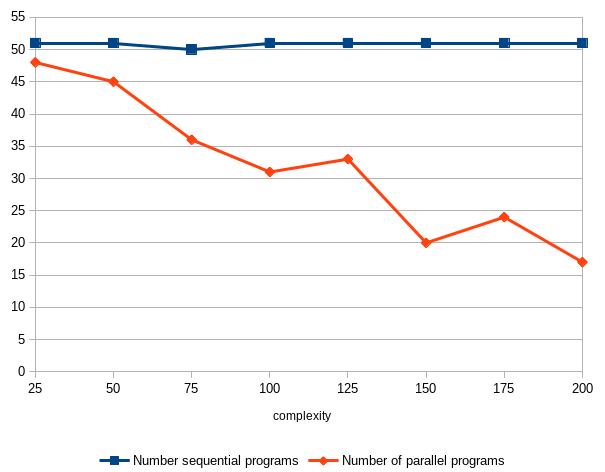
\includegraphics[width=0.8\textwidth]{img/generated/par-success-1.png}
    \caption{\label{fig:gen-par-success-1}Number of programs successfully parallelised for the first program set}
\end{figure}
\begin{figure}
    \centering
    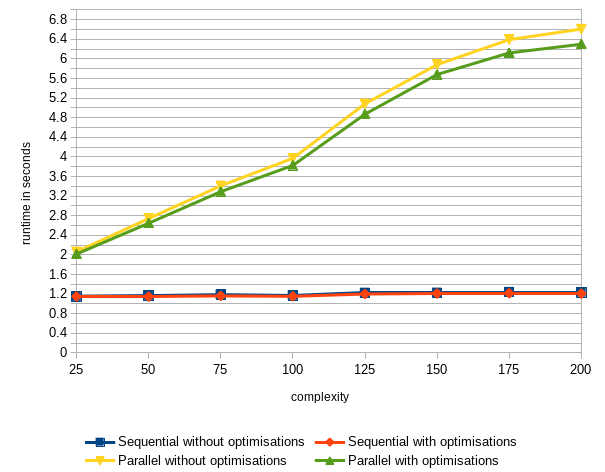
\includegraphics[width=0.8\textwidth]{img/generated/avg-runtime-1.png}
    \caption{\label{fig:gen-avg-runtime-1}Average runtime for the first program set}
\end{figure}
\begin{figure}
    \centering
    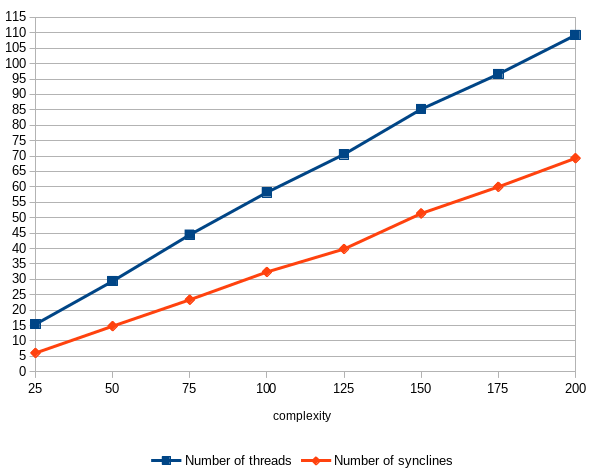
\includegraphics[width=0.8\textwidth]{img/generated/thread-count-1.png}
    \caption{\label{fig:gen-thread-count-1}Average number of threads and synclines for the first program set}
\end{figure}

\begin{figure}
    \centering
    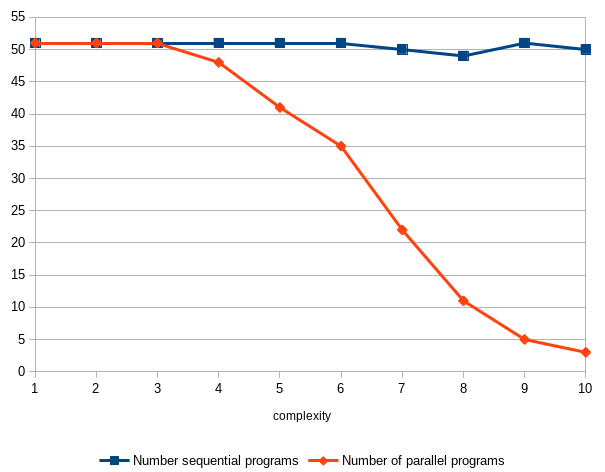
\includegraphics[width=0.8\textwidth]{img/generated/par-success-2.png}
    \caption{\label{fig:gen-par-success-2}Number of programs successfully parallelised for the second program set}
\end{figure}
\begin{figure}
    \centering
    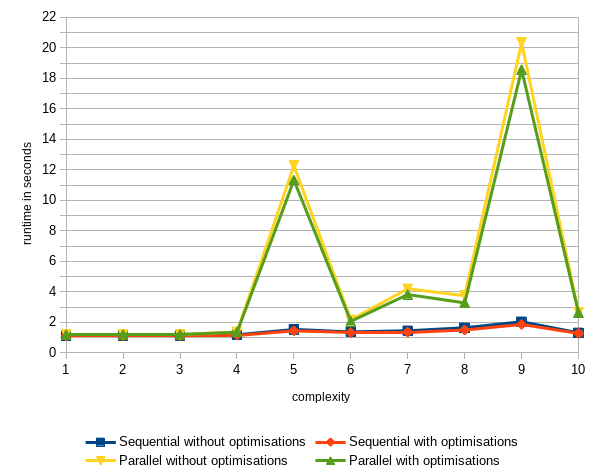
\includegraphics[width=0.8\textwidth]{img/generated/avg-runtime-2.png}
    \caption{\label{fig:gen-avg-runtime-2}Average runtime for the second program set}
\end{figure}
\begin{figure}
    \centering
    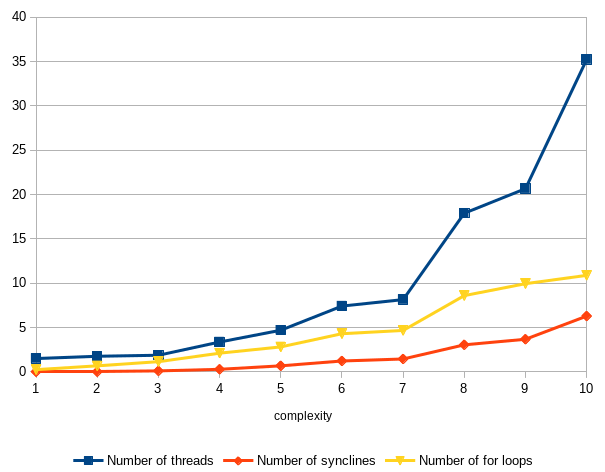
\includegraphics[width=0.8\textwidth]{img/generated/thread-count-2.png}
    \caption{\label{fig:gen-thread-count-2}Average number of threads and synclines for the second program set}
\end{figure}

\begin{figure}
    \centering
    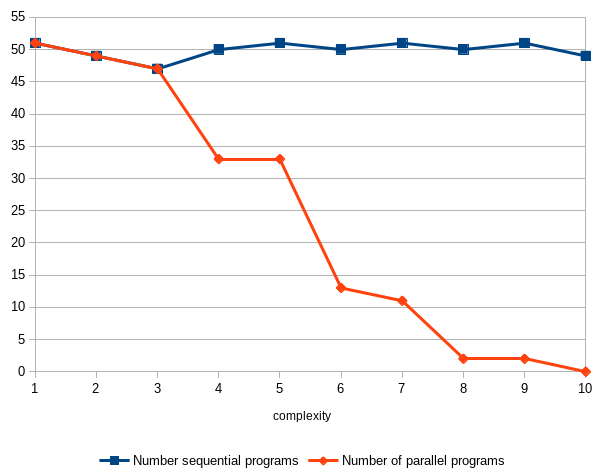
\includegraphics[width=0.8\textwidth]{img/generated/par-success-3.png}
    \caption{\label{fig:gen-par-success-3}Number of programs successfully parallelised for the third program set}
\end{figure}
\begin{figure}
    \centering
    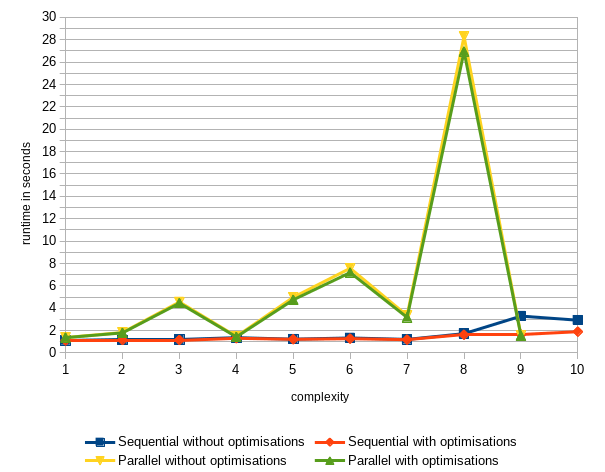
\includegraphics[width=0.8\textwidth]{img/generated/avg-runtime-3.png}
    \caption{\label{fig:gen-avg-runtime-3}Average runtime for the third program set}
\end{figure}
\begin{figure}
    \centering
    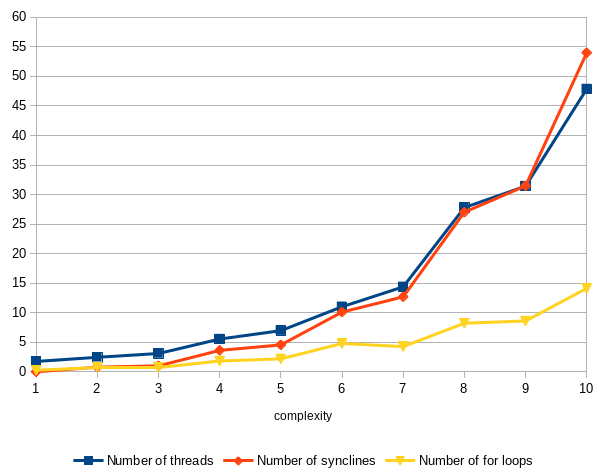
\includegraphics[width=0.8\textwidth]{img/generated/thread-count-3.png}
    \caption{\label{fig:gen-thread-count-3}Average number of threads and synclines for the third program set}
\end{figure}
